\documentclass{standalone}
    %
    \usepackage{tikz,xcolor}
    \usetikzlibrary{shapes.geometric,arrows,positioning,fit}
    
\begin{document}
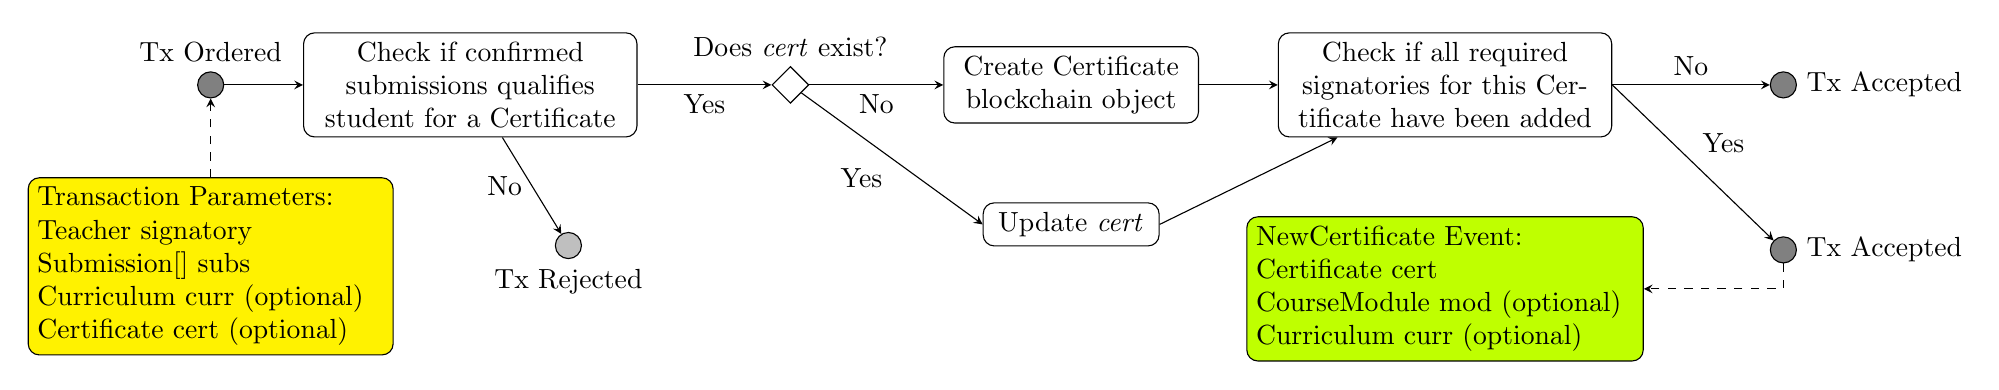
\begin{tikzpicture}[>=stealth,every node/.style={shape=rectangle,draw,rounded corners},]
	% create the nodes
	\node (start)[shape=circle, fill=gray, label=above:Tx Ordered] {};
	\node (param)[below =of start, text width=4.4cm, fill=yellow]{Transaction Parameters:\\Teacher signatory \\Submission[] subs\\ Curriculum curr (optional)\\ Certificate cert (optional)};
    \node (c1) [right =of start, text width=4cm, align=center]{Check if confirmed submissions qualifies student for a Certificate};
	\node (c1b) [shape=diamond, sharp corners, right = 1.7cm of c1, label=above: Does \textit{cert} exist?]{};    
    \node (c1c) [right = 1.7cm of c1b, text width=3cm, align=center]{Create Certificate blockchain object};    
	\node (c1d) [below =of c1c, text width=2cm, align=center]{Update \textit{cert}};        
	\node (c2) [right = of c1c, text width=4cm, align=center]{Check if all required signatories for this Certificate have been added};
	\node (stop1)[right = 2cm of c2, shape=circle, fill=gray, label=right:Tx Accepted] {};
    \node (stop2)[below = 1.75cm of stop1, shape=circle, fill=gray, label=right:Tx Accepted] {};
    \node (stop3)[below right = 1.25cm and -1cm of c1, shape=circle, fill=lightgray, label=below:Tx Rejected] {};    
    \node (event1)[below =of c2, text width=4.8cm, fill=lime]{NewCertificate Event:\\ Certificate cert\\CourseModule mod (optional)\\ Curriculum curr (optional) };    

	% connect the nodes
	\draw[->, dashed] (param) to (start);
	\draw[->] (start) to (c1);
    \draw[->] (c1) -- node[draw=none, anchor=north] {Yes} (c1b);
    \draw[->] (c1) -- node[draw=none, anchor=east] {No} (stop3);
    \draw[->] (c1b) -- node[draw=none, anchor=north] {No} (c1c);  
    \draw[->] (c1b) -- node[draw=none, anchor=north east] {Yes} (c1d.west);      
    \draw[->] (c1c) to (c2);                
	\draw[->] (c1d.east) to (c2);                        
	\draw[->] (c2) -- node[draw=none, anchor=south] {No} (stop1);
    \draw[->] (c2.east) -- node[draw=none, anchor=south west] {Yes} (stop2);
	\draw[->, dashed] (stop2) |- (event1.east);
    
\end{tikzpicture}
\end{document}
